\subsection{Архитектура клиентской части системы}

Клиентская часть разрабатываемой системы реализована в виде \textbf{одностраничного приложения (SPA)} с использованием фреймворка \textbf{Next.js}, поддерживающего гибкий рендеринг — как на стороне клиента (CSR), так и на стороне сервера (SSR). Такое решение позволяет обеспечить как высокую производительность и отзывчивость пользовательского интерфейса, так и оптимизацию индексации содержимого поисковыми системами за счёт серверного рендеринга.

\subsubsection{Общая структура архитектуры}

Для организации структуры проекта был применён подход \textbf{Feature-Sliced Design (FSD)} — современная парадигма проектирования front-end приложений, ориентированная на модульность, масштабируемость и соответствие предметной области. В отличие от традиционных архитектур, основанных на технических слоях (например, разделение на компоненты, страницы или сервисы), FSD предполагает смысловое разделение приложения на функциональные модули, которые отражают реальные пользовательские сценарии и бизнес-логику.

Каждый модуль FSD отвечает за строго ограниченную область и содержит всё необходимое для своей работы: представление, поведение, взаимодействие с API и внутренние модели. Это способствует повышению читаемости и повторному использованию кода, а также упрощает сопровождение и развитие системы в долгосрочной перспективе.

\subsubsection{Архитектурная диаграмма}

\begin{figure}[H]
\centering
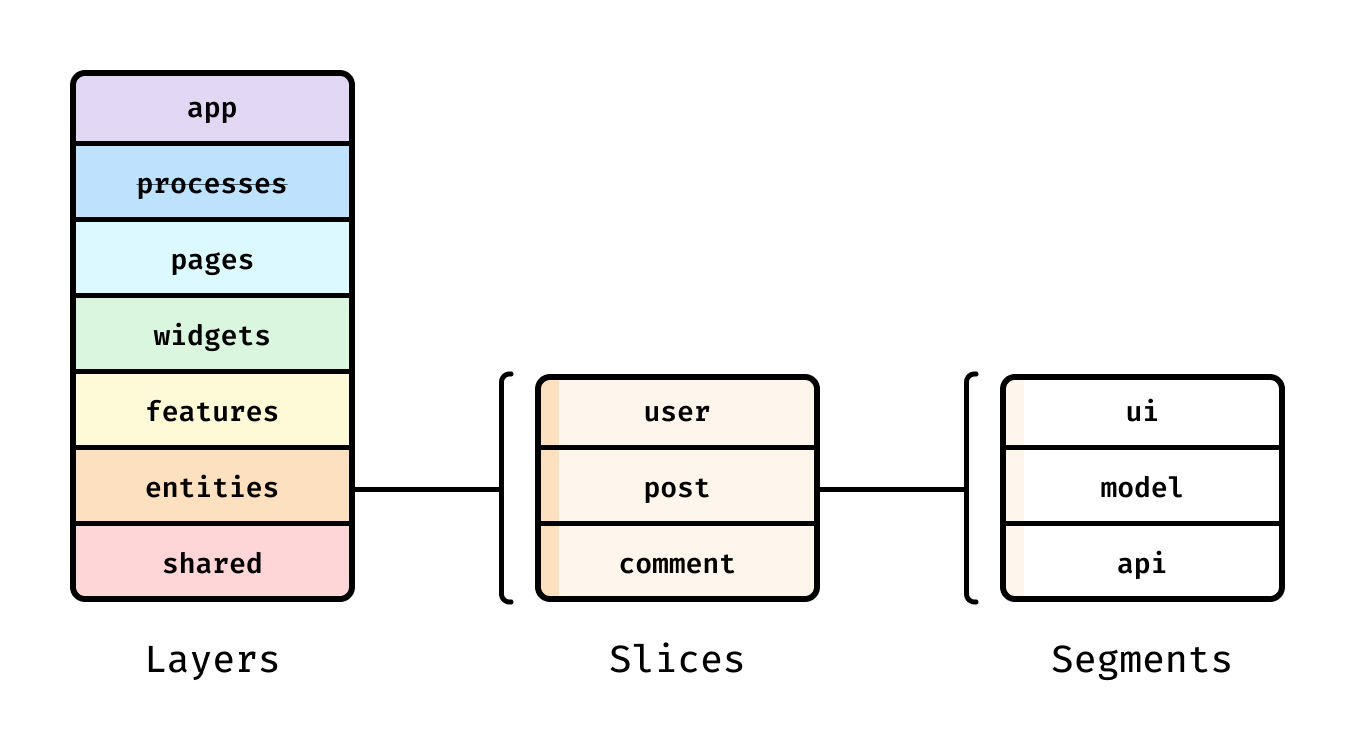
\includegraphics[width=0.7\linewidth]{static/fsdImage}
\caption{Схема архитектуры клиентской части (FSD + Next.js)}
\end{figure}

На диаграмме представлены основные уровни и элементы архитектуры приложения. Следует отметить, что каждый слой в данной структуре ориентирован на строгое разграничение ответственности. Компоненты нижних уровней не имеют информации о вышестоящих слоях, что позволяет реализовать принцип инверсии зависимостей и минимизировать связанность между модулями.

\subsubsection{Слои архитектуры Feature-Sliced Design}

\begin{table}[H]
\centering
\caption{Слои архитектуры Feature-Sliced Design}
\begin{tabular}{|p{3cm}|p{11cm}|}
\hline
\textbf{Слой} & \textbf{Описание и назначение} \\
\hline
\texttt{app} & Точка входа в приложение: глобальные стили, маршрутизация, провайдеры состояния, интеграции с внешними сервисами. \\
\hline
\texttt{pages} & Страницы, связанные с маршрутизацией. Формируются из виджетов и не содержат бизнес-логики. \\
\hline
\texttt{widgets} & Крупные элементы интерфейса, отражающие пользовательские сценарии, например, чат, список заданий, панель управления. \\
\hline
\texttt{features} & Изолированные пользовательские функции, такие как авторизация, отправка сообщений или регистрация. Могут включать бизнес-логику и вызовы API. \\
\hline
\texttt{entities} & Базовые предметные сущности предметной области, включающие типы, схемы, API и UI-представление. \\
\hline
\texttt{shared} & Универсальные компоненты, утилиты и типы, переиспользуемые во всём проекте. \\
\hline
\end{tabular}
\end{table}

\subsubsection{Концепция срезов (slices)}

Ключевым элементом архитектурного подхода Feature-Sliced Design является понятие \textbf{срезов} (англ. \textit{slices}). Под срезом понимается логически обособленный модуль, реализующий завершённую часть функциональности приложения. Каждый срез может содержать собственные модели данных, визуальные компоненты, бизнес-логику, а также механизмы взаимодействия с внешними источниками данных.

Срезы группируются по смысловому признаку и могут располагаться в рамках различных уровней архитектуры: \texttt{features}, \texttt{entities}, \texttt{widgets}, \texttt{pages}. Такое структурирование обеспечивает лучшую декомпозицию кода, повышает его читабельность и облегчает модульное тестирование.

Например:
\begin{itemize}
  \item \texttt{features/login} — срез, реализующий сценарий авторизации пользователя;
  \item \texttt{entities/task} — срез, содержащий всё, что связано с сущностью «задание»;
  \item \texttt{widgets/ChatWindow} — срез, объединяющий функциональность и интерфейс чат-интерфейса;
  \item \texttt{pages/home} — срез, реализующий главную страницу приложения.
\end{itemize}

Таким образом, построение приложения через срезы позволяет выстраивать архитектуру, ориентированную не на реализацию, а на назначение функциональных компонентов, что делает проект удобным для масштабирования и сопровождения.

\subsubsection{Горизонтальное деление на сегменты (segments)}

Каждый срез, независимо от своего уровня, может быть дополнительно разделён на \textbf{сегменты} (англ. \textit{segments}) — логические подкатегории, структурирующие содержимое среза по назначению кода. В отличие от слоёв, которые представляют вертикальную иерархию, сегменты формируют горизонтальное деление и обеспечивают внутреннюю организацию модулей.

Наиболее распространённые типы сегментов включают:
\begin{itemize}
  \item \texttt{ui} — визуальные компоненты и стили, определяющие отображение данных;
  \item \texttt{model} — модели данных, хранилища состояния, типизация и бизнес-логика;
  \item \texttt{api} — функции для работы с внешними сервисами, включая описание типов запросов и маппинг ответов;
  \item \texttt{lib} — вспомогательные функции и библиотеки, используемые в пределах данного среза;
  \item \texttt{config} — конфигурационные файлы и переключатели функциональности (feature flags).
\end{itemize}

Такой подход обеспечивает предсказуемую структуру каждого среза, делает код самодокументируемым и способствует упрощению навигации в большом проекте. Также, при необходимости, разработчики могут вводить дополнительные сегменты в рамках слоёв \texttt{shared} или \texttt{app}, не нарушая целостности архитектуры.

\subsubsection*{Преимущества выбранного подхода}

Применение архитектуры Feature-Sliced Design в контексте разрабатываемого клиентского приложения позволило достичь следующих результатов:

\begin{itemize}
  \item Чёткое разграничение обязанностей между модулями и слоями;
  \item Улучшенная масштабируемость проекта без деградации структуры;
  \item Повышенная модульность, обеспечивающая лёгкость в тестировании и повторном использовании кода;
  \item Создание условий для быстрой и эффективной интеграции новых членов команды в разработку;
  \item Архитектура, ориентированная на задачи и бизнес-логику, а не на технические детали.
\end{itemize}

В совокупности данные свойства делают архитектурное решение устойчивым к росту функциональности, улучшая поддержку и развитие системы в долгосрочной перспективе.
